\documentclass[11pt]{article}

\usepackage{amsmath,setspace,mathtools,amssymb,booktabs,graphicx, multicol}

\usepackage[utf8]{inputenc}

\usepackage[letterpaper,portrait,margin=0.5cm]{geometry}

\graphicspath{ {./} }


\title{Computational Physics Midterm}

\author{Thaseus Karkabe-Olson}

\date{}

\begin{document}
	
	
	\maketitle
	
	\begin{multicols}{2}

	\begin{center}

	\section*{Model Description}

	\end{center}

		\indent This model is set up to simulate how a number of cars n behave on a ring road given several initial conditions. These include driver reaction times,the length of vehicles, the size of the road,
		the desired speed of the drivers, and the initial positions and velocities of cars.

		\indent From this we can find out how the cars actually move. We accomplish this by calculating the rates of change for both velocity and position of each car using the differential equation
		from the IDM model. Utilizing ODEint we can then solve for our resulting velocities and positions at each point in time along a given time interval. From there, we then simply plot our positions and
		velocities of each car to see how they behave over time. Here is an example of how 50 cars behave when spaced apart evenly and with random initial velocities:
	
		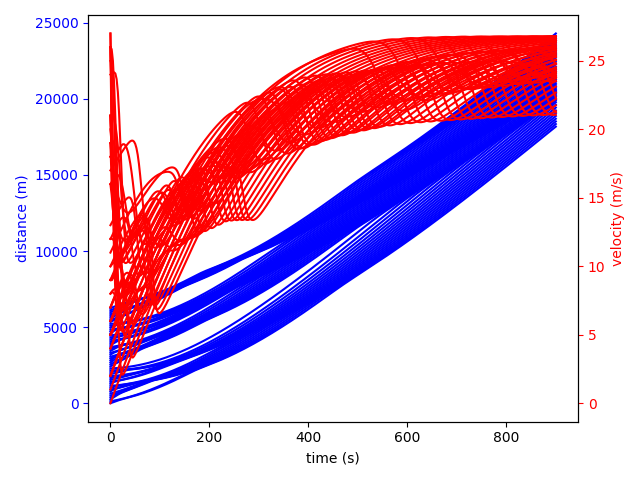
\includegraphics[scale = 0.5]{Figure_1.png}

		\indent You can see from this graph that we get two results: velocity and position over time for each car. Blue coorisponds to how far in total each car moves in metres, while the red coorisponds
		to what the velocity at a given time is for each car in metres per second.

	\begin{center}

	\section*{Experiments}

		\subsection*{Equilibrium Speed}

	\end{center}

		\indent Here is another example of a setup, this time where all cars start at the same speed except the first and where we have a smaller road and less cars

		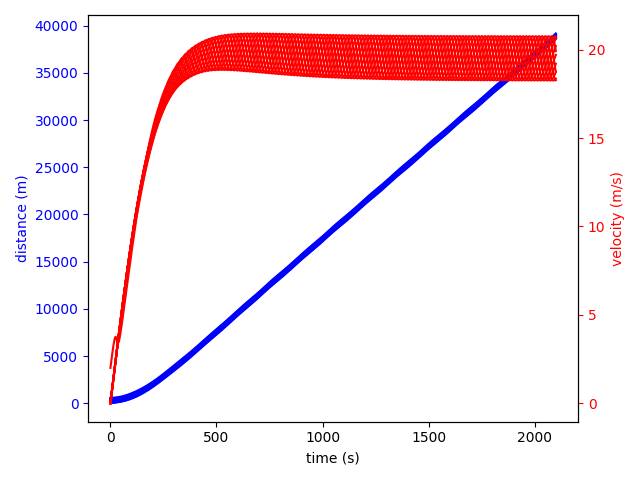
\includegraphics[scale = 0.5]{Figure_2.png}

	\end{multicols}


\end{document}
